\subsubsection{Requirements: } 
Infantile cardiac surgery offers a reconfiguration of the blood vessel walls that limits or rectifies the congenital anomalies of the anatomy.
During the surgery, the vessel walls are deformed, cut, and reconnected to other vessels.
To do a planning of the surgery, the geometry changes of these vessel walls (the motions and deformations, their configuration when they are cut or stitched)  must be anticipated.

These requirements ask for a physics-based model for the vessel walls. 
This model should provide 
(I) a good support for the deformations by bending and twisting. 
(II) an accurate modeling of the wall motion when the vessel is cut along its axis 
(III) global deformations of stitched vessels that capture their final configuration, after surgery 
(IV) collision response when detected (e.g. between the aortic arch and pulmonary artery). 

In addition, the computation of this model must be fast enough to allows for interactive planning of the surgery. 
The options on the choice of model are limited: 
The model based on the deformation of the centerline, that can be very quickly computed, (like ??\tomas{Add refs.!} \christian{Do you have some refs that uses model based on centerline? }\tomas{No, but I will find something}  ) must be discarded because they do not support cut of the wall along the vessel axis. 
Mass-springs approaches that are often used for cloth simulation \cite{Volino2005b}, allow for fast computation but do not provide sufficient accuracy as they do not necessary converge to a unique solution when changing the mesh.
In this work, we then propose to rely on Finite Element formulation of thin-shell theory. 
These model are numerically more expensive, but provide accurate models of thin deformable structure.% that converge to unique solutions.
Moreover, we show that we can still obtain fast computation with a reasonable number of elements.


\subsubsection{Thin shell elements: } 
The formulation of the thin shell elements is based on the mechanics of continuum. 
For thorough description we refer the reader to the textbook about Finite Element methods for example \cite{Reddy1993}.
These elements are commonly used in physics and mechanics for deformation modelling of thin structures because they are numerically more stable then volumetric FEM methods in this situation. 
The shell element is a 2-dimensional element (in our case, triangular element) whose thickness is a parameter of the simulation (often considered constant over the surface of the element).
Shell element combines forces from in-plane deformations, like stretching or shearing, with bending forces. 
Such internal forces $\myvec{f}$ are a function of current displacement measured as difference of current shape
$\myvec{x}$ from the rest shape $\myvec{x_0}$.
To accelerate the computation, we use a corotational formulation, that is based on the definition of a local frame for each element (that can be built using the geometry of the triangle, \christian{see figure "image: single shell" ?? }). 

In this local frame, the computation of the internal forces is linear:
\begin{equation}
  \myvec{f} = \mathbf{K_e}(\myvec{x} - \myvec{x_0})
 \label{linear_static_model} 
\end{equation}
where $\mymat{K_e}$ is a stiffness matrix that is computed thanks to a weak formulation (integral formulation) of Kirshohoff-Loves equations.
This approach is very similar to the model presented in  \cite{Comas2010b,Comas2010c}  even if the interpolation functions we use are  different to allow for better convergence\footnote{Our shell model will be published separately}. 
We emphasize that the method described in the paper is independent of the shell model used (other non-corotational shell models can be used as well).
%
When the structure is assembled, the contributions of each element are computed in the global frame using a different rotation matrix for each element.
\begin{equation}
\mathbb{K} = \mathcal{A}_{e=0}^N (\mathbf{R_e}^T \mathbf{K_e} \mathbf{R_e}) \hspace{10mm}
\mathbb{F} = \mathcal{A}_{e=0}^N ( \mathbf{R_e}^T \mathbf{K_e}(\myvec{x} - \myvec{x_0}))
\end{equation}
Where $\mathcal{A}$ is the assembling operator over the $N$ elements of the mesh, $\mathbb{K}$ is the global stiffness and $\mathbb{F}$ the internal forces of the entire shell mesh structure. 
Using this approach, $\mathbb{K}$ is changing at each step of the simulation but the model is able to catch geometric non-linear deformations.
In practice, the computation of the node motion $\mathbb{U} = \mathbb{K}^{-1} \mathbb{F}$ is performed using an optimized conjugate gradient algorithm.


\subsubsection{Accuracy: } 
In the following of the section we want to show that the performance of a model
based on shell elements is adequate for the simulation.

\begin{figure}[tbh]
  \begin{minipage}[b]{0.3\linewidth}
      \framebox[1cm]{\rule{0pt}{1cm}}
      %\includegraphics[width=\columnwidth]{img/}
      \caption{Bending shell element}
      \label{fig-shell}
  \end{minipage}
  \hspace{0.1\columnwidth}
  \begin{minipage}[b]{0.6\linewidth}
    \centering
    \begin{tabular}{cc}
     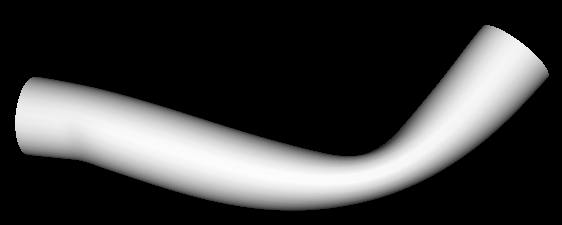
\includegraphics[width=0.5\columnwidth]{img/compare-bend.png}
      &
      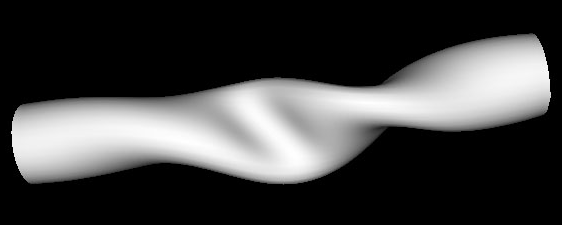
\includegraphics[width=0.5\columnwidth]{img/compare-twist.png}
      \\
      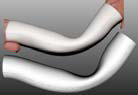
\includegraphics[width=0.5\columnwidth]{img/compare-bend-other.png}
      &
      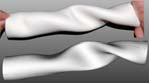
\includegraphics[width=0.5\columnwidth]{img/compare-twist-other.png}
    \end{tabular}
    \caption{Bending and twisting deformations. Upper: shell model; middle:
    artificial tube, bottom: Cosserat rod \cite{Li2009}. (Credits for the
    bottom images: Li et al.)}
    \label{fig-deformations}
  \end{minipage}
\end{figure}

Figure \ref{fig-deformations} shows bending and twisting deformations.
These are likely to occur during the surgery.
The figure compares our
results with the results of Li et al. \cite{Li2009}. As you can see the
results are close to the real deformations.

The bending property of the shell allows us to use smaller number of
elements for the simulation and use high polygonal model only for
visualisation. The convergence of the model is a key factor here. In our
experiments we were able to use only as few as eight nodes around the
circumference of a tubular model while still maintaining realistic
behaviour. Figure \ref{fig-convergence} shows the results for different
number of nodes along the circumference.

\begin{figure}[tbh]
  \centering
  \begin{tabular}{cccc}
    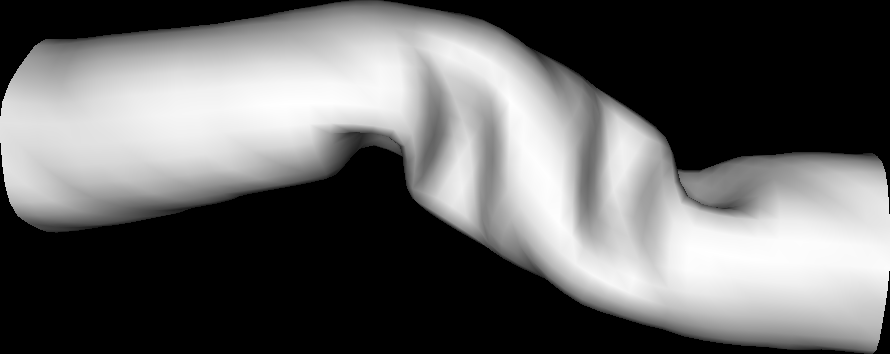
\includegraphics[width=0.24\columnwidth]{img/twist-06-cg.png}
    &
    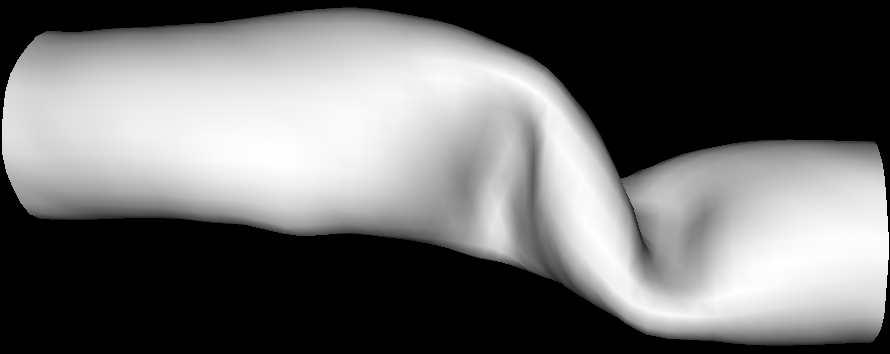
\includegraphics[width=0.24\columnwidth]{img/twist-08-cg.png}
    &
    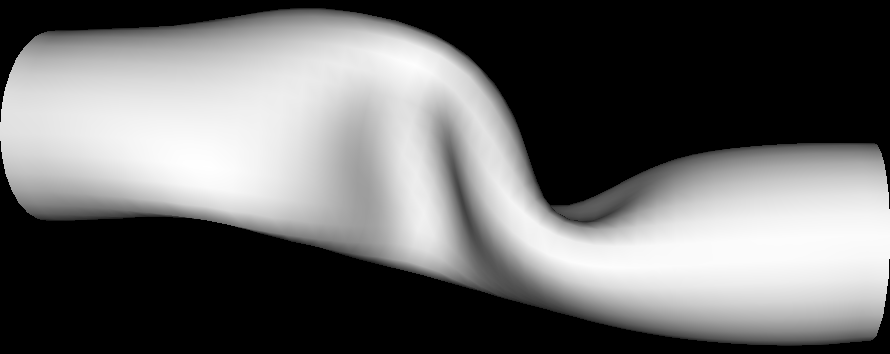
\includegraphics[width=0.24\columnwidth]{img/twist-16-cg.png}
    &
    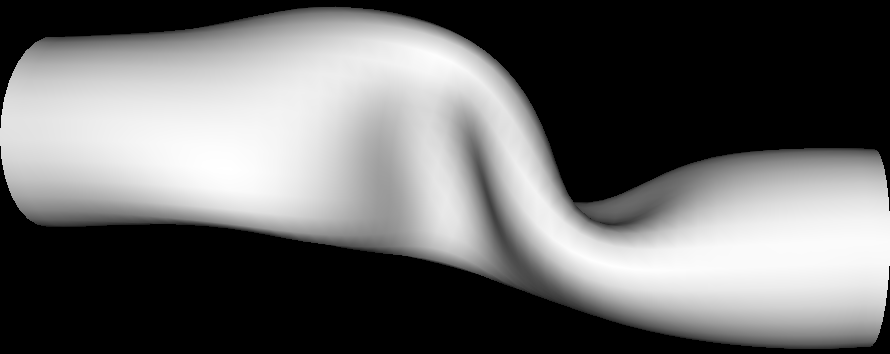
\includegraphics[width=0.24\columnwidth]{img/twist-31-cg.png}
    \\
    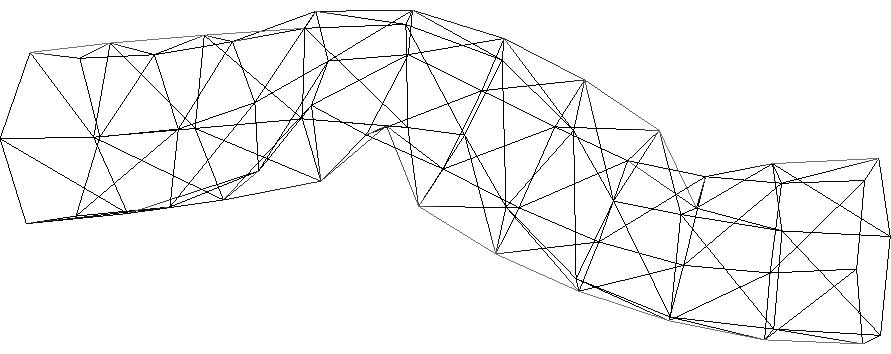
\includegraphics[width=0.24\columnwidth]{img/twist-06w-cg.png}
    &
    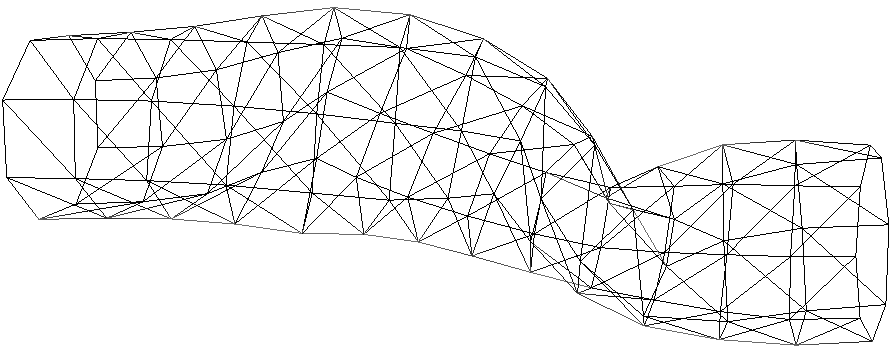
\includegraphics[width=0.24\columnwidth]{img/twist-08w-cg.png}
    &
    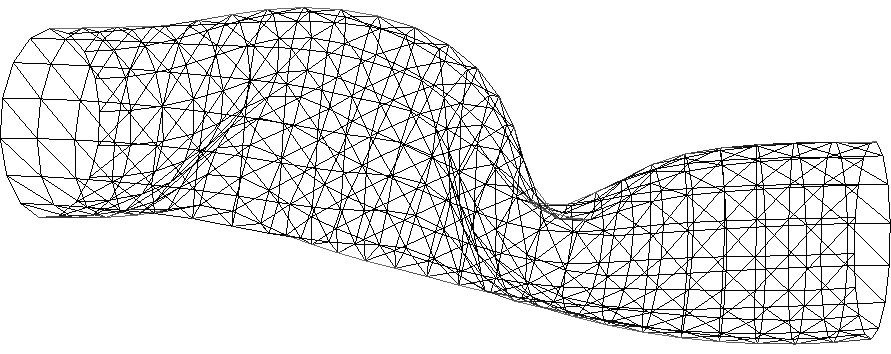
\includegraphics[width=0.24\columnwidth]{img/twist-16w-cg.png}
    &
    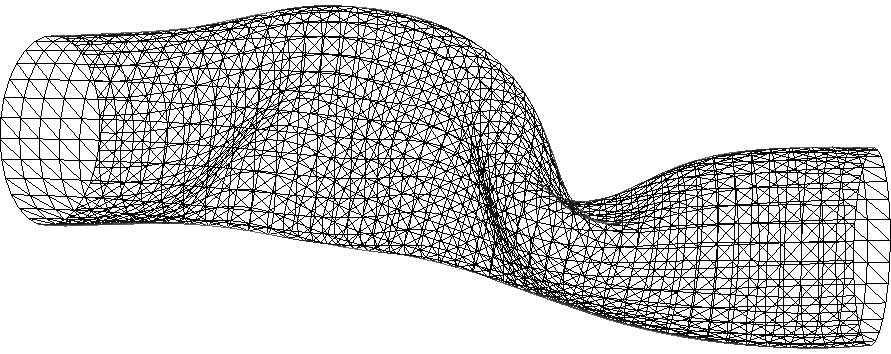
\includegraphics[width=0.24\columnwidth]{img/twist-31w-cg.png}
  \end{tabular}
  \caption{Convergence on a twisted cylinder with 6, 8, 16 and 31 nodes
  around the circumference (120, 208, 832 and 3038 elements).
  Using mesh with 3038 triangles for visualisation.
  \tomas{improve the wireframe images if there's time} } 
  \label{fig-convergence}
\end{figure}



\christian{ I think this should be put in the result section:
Since we use the method as a
geometrical tool we have also certain independence on physical parameters.
For example the variation of Young's modulus in the interval from $10^3$ to
$10^7$ resulted in only $0.1\%$ change of the deformation.
}


% vim: et sw=2 tw=0 spell
